\documentclass[12pt, a4paper]{article}

% ── Packages ──
\usepackage[margin=1in, headheight=14.5pt]{geometry}
\usepackage{graphicx}
\usepackage{float}
\usepackage{hyperref}
\usepackage{booktabs}
\usepackage{enumitem}
\usepackage{titlesec}
\usepackage{fancyhdr}
\usepackage{caption}
\usepackage{subcaption}
\usepackage{array}
\usepackage{xcolor}
\usepackage{tabularx}
\usepackage{amsmath}

% ── Graphics path ──
\graphicspath{{../Gallery/}}

% ── Hyperlink styling ──
\hypersetup{
    colorlinks=true,
    linkcolor=blue!70!black,
    urlcolor=blue!60!black,
    citecolor=blue!70!black,
    pdftitle={Thelawala - A Vendor Aggregation Platform},
    pdfauthor={Anurag Sharma, Parth Pandey, Grishmank Parate, Shashwat Kumar Chandan}
}

% ── Fix duplicate page.1 identifier ──
\hypersetup{pageanchor=false}

% ── Header / Footer ──
\pagestyle{fancy}
\fancyhf{}
\rhead{Thelawala --- Mid Semester Review}
\lhead{IIITDM Kancheepuram}
\cfoot{\thepage}

% ── Title formatting ──
\titleformat{\section}{\Large\bfseries}{\thesection.}{0.5em}{}
\titleformat{\subsection}{\large\bfseries}{\thesubsection}{0.5em}{}

\begin{document}

% ═══════════════════════════════════════════════════
% TITLE PAGE
% ═══════════════════════════════════════════════════
\begin{titlepage}
    \centering
    \vspace*{1cm}

    {\large\bfseries Indian Institute of Information Technology,}\\[0.15cm]
    {\large\bfseries Design \& Manufacturing, Kancheepuram}\\[1.2cm]

    \rule{\linewidth}{0.4pt}\\[0.6cm]

    {\Huge\bfseries Thelawala}\\[0.4cm]
    {\LARGE A Vendor Aggregation Platform}\\[0.6cm]

    \rule{\linewidth}{0.4pt}\\[1.2cm]

    {\large\textbf{Mid Semester Review}}\\[0.3cm]
    {\large DS3001 --- Prototyping \& Testing}\\[2cm]

    \begin{tabular}{l l}
        \toprule
        \textbf{Roll Number} & \textbf{Name} \\
        \midrule
        CS23B1062  & Anurag Sharma \\
        CS23I1064  & Parth Pandey \\
        CS23I1026  & Grishmank Parate \\
        ME23B1009  & Shashwat Kumar Chandan \\
        \bottomrule
    \end{tabular}\\[1.5cm]

    {\large \textbf{Mentor:} Dr.\ Narendran G.}\\[1cm]

    {\large March 2026}

    \vfill
\end{titlepage}

\hypersetup{pageanchor=true}
\tableofcontents
\newpage

% ═══════════════════════════════════════════════════
% 1. PROBLEM STATEMENT
% ═══════════════════════════════════════════════════
\section{Problem Statement}

Street vendors --- commonly known as \textit{thelawalas} --- form a significant part of India's informal economy. Despite serving millions of customers daily, their operations remain entirely invisible in the digital space. Buyers have no way of knowing:

\begin{itemize}[noitemsep]
    \item When or where a specific vendor will appear in their locality.
    \item What products a nearby vendor is currently selling.
    \item Whether a vendor they prefer is even operating on a given day.
\end{itemize}

This unpredictability leads to missed purchase opportunities for buyers and lost revenue for vendors. Furthermore, no structured communication channel exists between a buyer and a thelawala --- a buyer cannot signal purchase intent, and a vendor cannot notify regular customers of their presence.

From a vendor's perspective, thelawalas lack any digital tool tailored to their trade. Existing platforms (food delivery apps, ride-hailing services) are designed for formal businesses and do not map to the mobile, informal, and low-capital nature of street vending. Additionally, many thelawalas do not own a smartphone, making any phone-dependent GPS solution impractical for continuous all-day use.

\textbf{In summary:} the street-vending ecosystem suffers from a lack of real-time location awareness, product discoverability, and bidirectional communication --- problems that no existing platform addresses.

% ═══════════════════════════════════════════════════
% 2. OBJECTIVES
% ═══════════════════════════════════════════════════
\section{Objectives}

The primary objective of this project is to design and build a platform that bridges the information gap between street vendors and local buyers. The specific objectives are:

\begin{enumerate}[noitemsep]
    \item \textbf{Real-time vendor tracking:} Enable buyers to see the live location of nearby thelawalas on a map.
    \item \textbf{Product-level discovery:} Allow buyers to search for vendors selling a specific item (e.g., ``panipuri'') and see results filtered by proximity.
    \item \textbf{Buyer--vendor communication:} Provide a structured request mechanism where a buyer can request an item from a vendor, relaying their location so the vendor can approach them.
    \item \textbf{Hardware independence:} Design a dedicated low-power GPS device (AUJAR) that can broadcast a vendor's location without requiring them to own or operate a smartphone.
    \item \textbf{Proximity notification:} Notify users when a subscribed vendor enters their vicinity, even when the app is not active, through automated calling services.
\end{enumerate}

% ═══════════════════════════════════════════════════
% 3. ASSUMPTIONS
% ═══════════════════════════════════════════════════
\section{Assumptions}

The following assumptions were made during the design and development of the system:

\begin{enumerate}[noitemsep]
    \item Buyers (users) have access to an Android smartphone with GPS and internet connectivity.
    \item The server has a stable internet connection and is reachable from the mobile applications.
    \item Vendors may or may not own a smartphone; the system accounts for both scenarios through the AUJAR hardware device.
    \item In the current prototype phase, the vendor's mobile phone GPS substitutes for the AUJAR device's GPS module.
    \item All parties operate within a geographically bounded area where cellular data or Wi-Fi connectivity is available.
    \item Vendors are willing to broadcast their location in exchange for increased customer visibility and sales.
\end{enumerate}

% ═══════════════════════════════════════════════════
% 4. CONCEPT DESIGN
% ═══════════════════════════════════════════════════
\section{Concept Design}

\subsection{Research-Driven Focus Areas}

The concept design was driven by structured analysis using three frameworks:

\textbf{SNAC Analysis} identified four critical pain points in the street-vending ecosystem: unpredictable vendor availability, absence of any communication channel between buyers and vendors, complete vendor invisibility in the digital space, and missed revenue due to buyers being unaware of nearby vendors.

\textbf{Discovery Matrix} mapped unmet needs against existing alternatives and confirmed that no real-time tracking solution exists for informal street vendors, product-level search is entirely absent, and bidirectional buyer--vendor communication is an unaddressed gap.

\textbf{Interpretive Structural Modelling (ISM)} established a hierarchy of driving and dependent factors. Vendor location awareness, real-time communication infrastructure, and low-barrier hardware access emerged as foundational drivers (high driving power, low dependence), while purchase conversion, customer satisfaction, and vendor income growth were identified as dependent outcomes.

The convergent conclusion: the solution must focus on \textbf{(1) real-time vendor location tracking}, \textbf{(2) product discovery}, and \textbf{(3) a structured buyer--vendor communication channel}.

\subsection{Core Concept}

The platform provides four key capabilities:

\begin{enumerate}[noitemsep]
    \item \textbf{Track} --- A user can see the live location of thelawalas on a map.
    \item \textbf{Discover} --- A user can view all vendors broadcasting near their current location.
    \item \textbf{Search} --- A user can search for vendors selling a specific product (by item name or vendor ID).
    \item \textbf{Request} --- A user can send a purchase request to a vendor; the buyer's location is relayed to the vendor, who can accept or reject the request.
\end{enumerate}

\subsection{Addressing Hardware Constraints --- The AUJAR Device}

Continuous GPS tracking drains a smartphone's battery rapidly, and many thelawalas do not own a smartphone. To address both constraints, the concept introduces \textbf{AUJAR} --- a purpose-built, low-power hardware device:

\begin{itemize}[noitemsep]
    \item Contains a GPS module that continuously acquires the vendor's position.
    \item Transmits coordinates over Bluetooth Low Energy (BLE) to any paired smartphone nearby.
    \item The paired phone acts as a bridge, forwarding GPS data to the Thelawala server.
    \item Requires no interaction from the vendor --- simply turn on and mount on the thela.
    \item Designed to last a full work shift (8--12 hours) on a single charge.
\end{itemize}

\begin{figure}[H]
    \centering
    \begin{subfigure}[b]{0.48\textwidth}
        \centering
        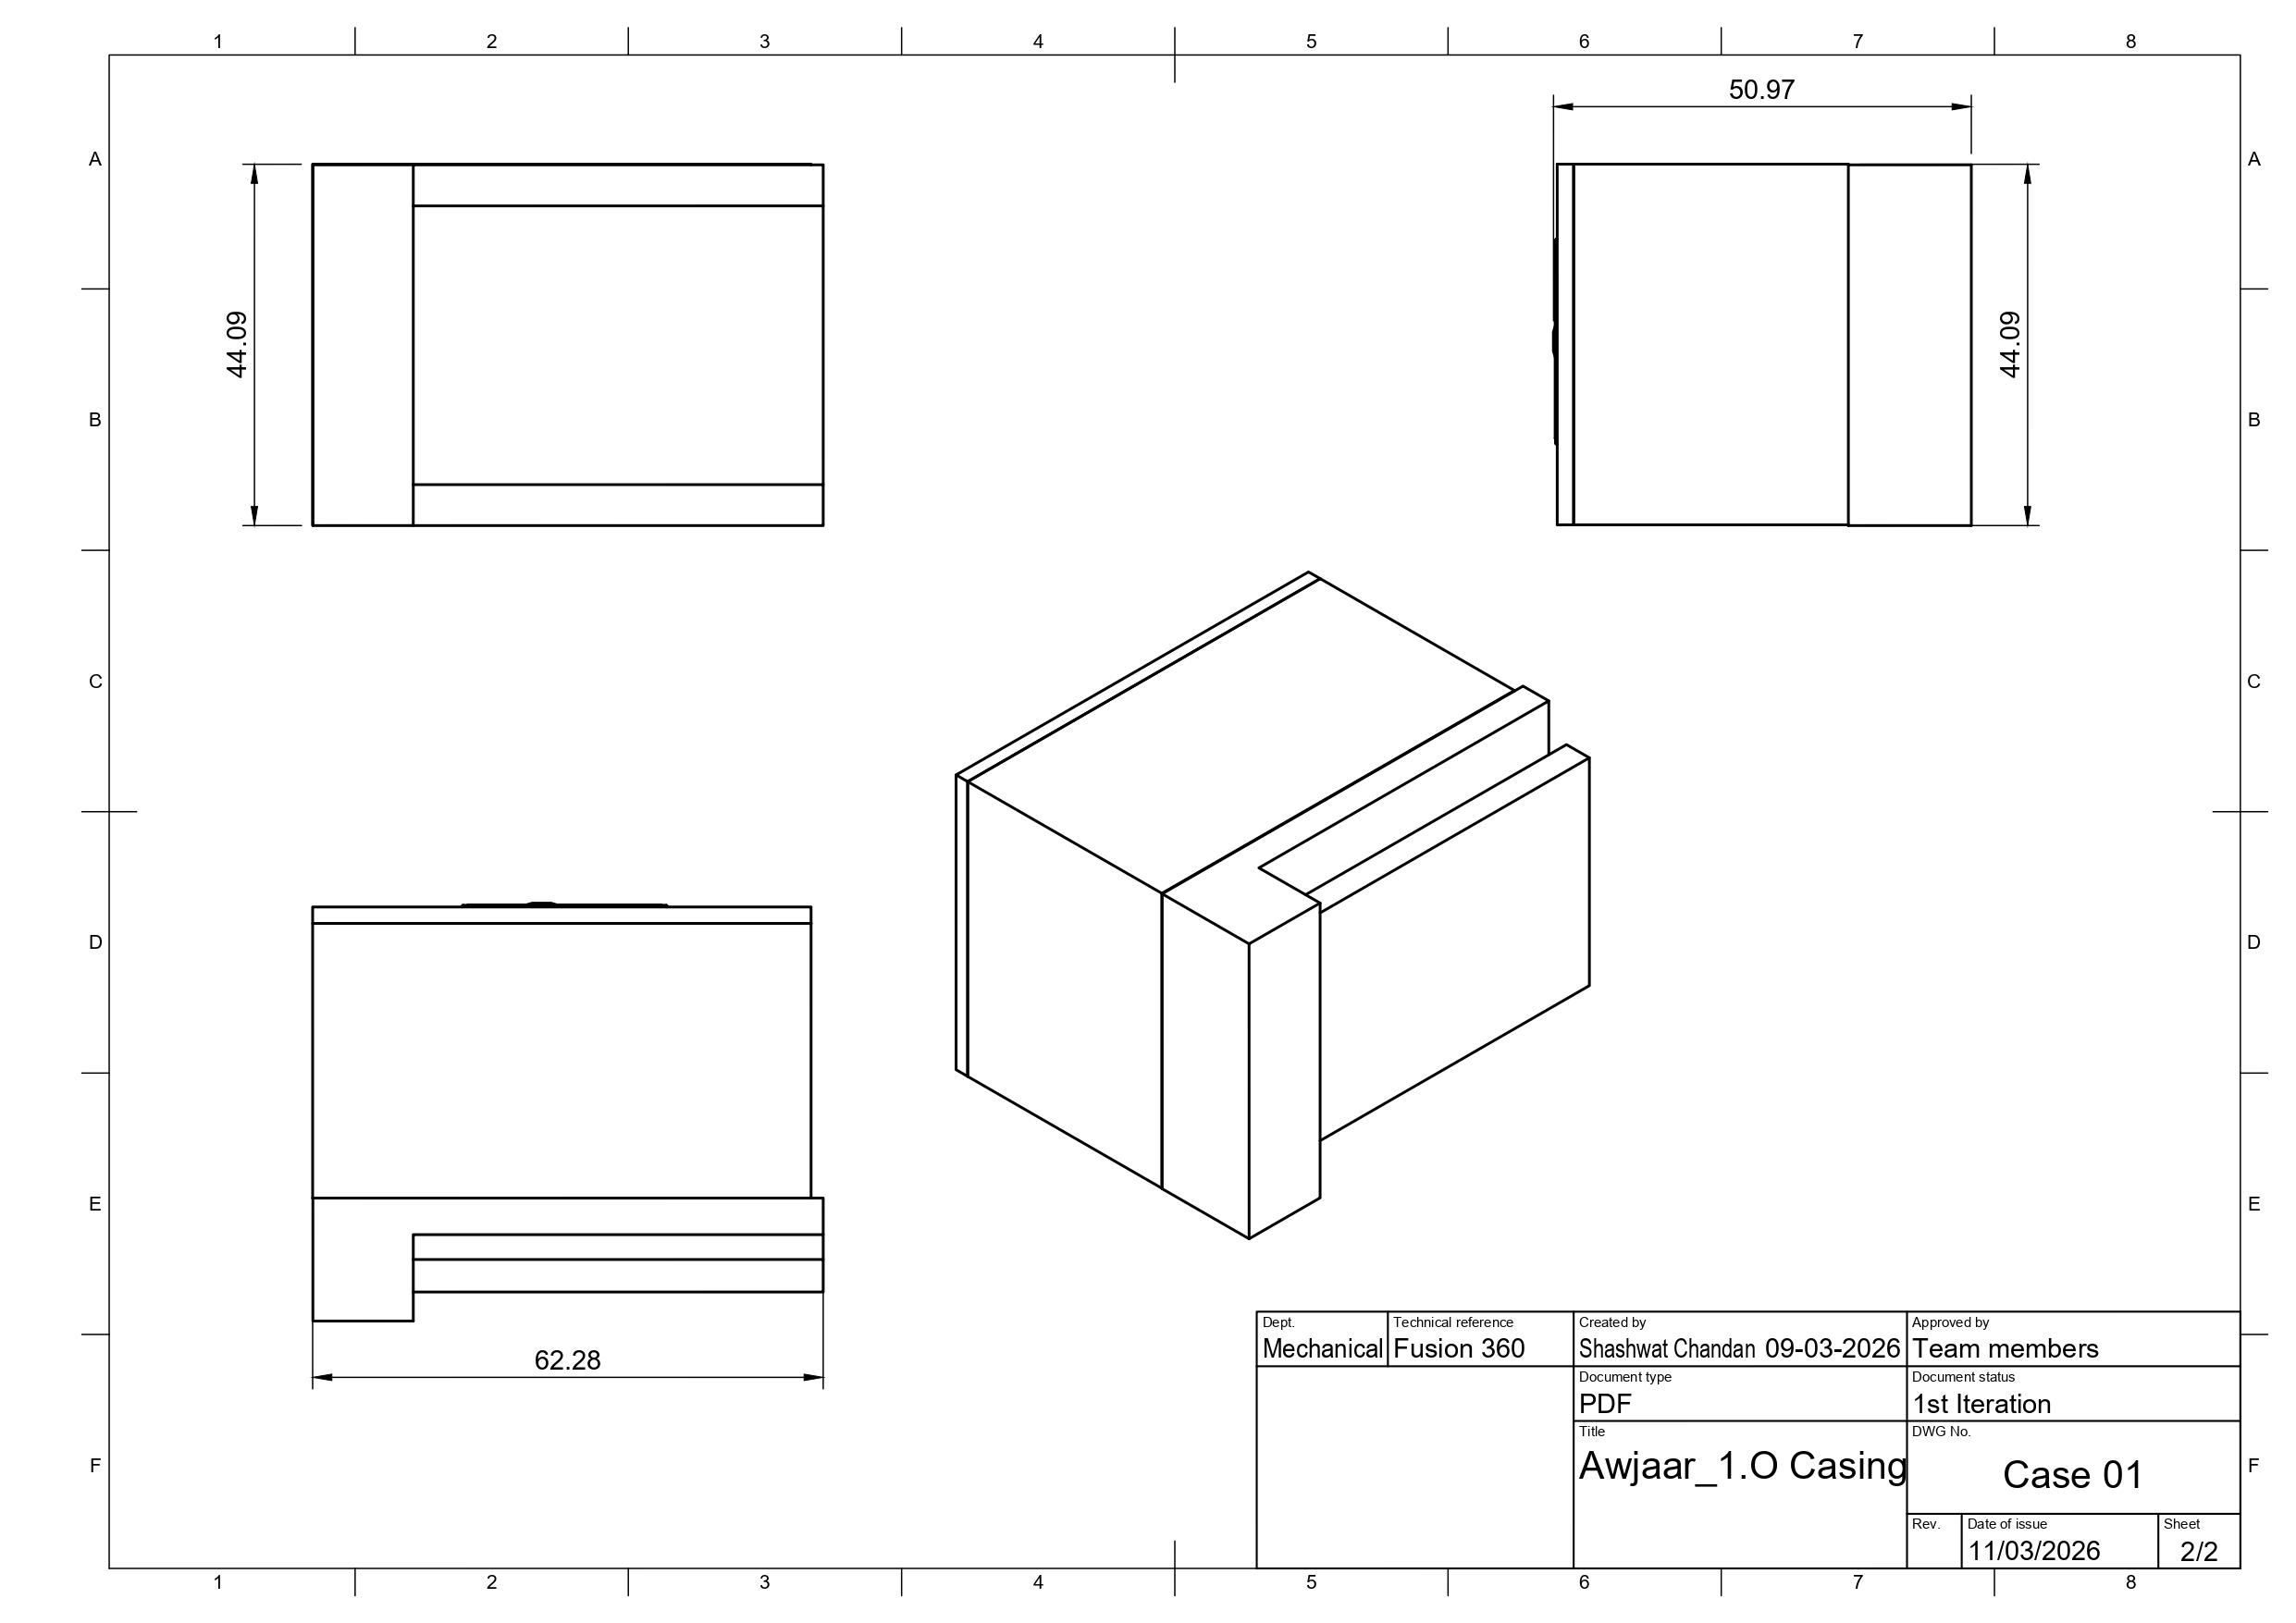
\includegraphics[width=\textwidth]{aujaar_2D_Casing.jpg}
        \caption{AUJAR 2D casing design}
    \end{subfigure}
    \hfill
    \begin{subfigure}[b]{0.48\textwidth}
        \centering
        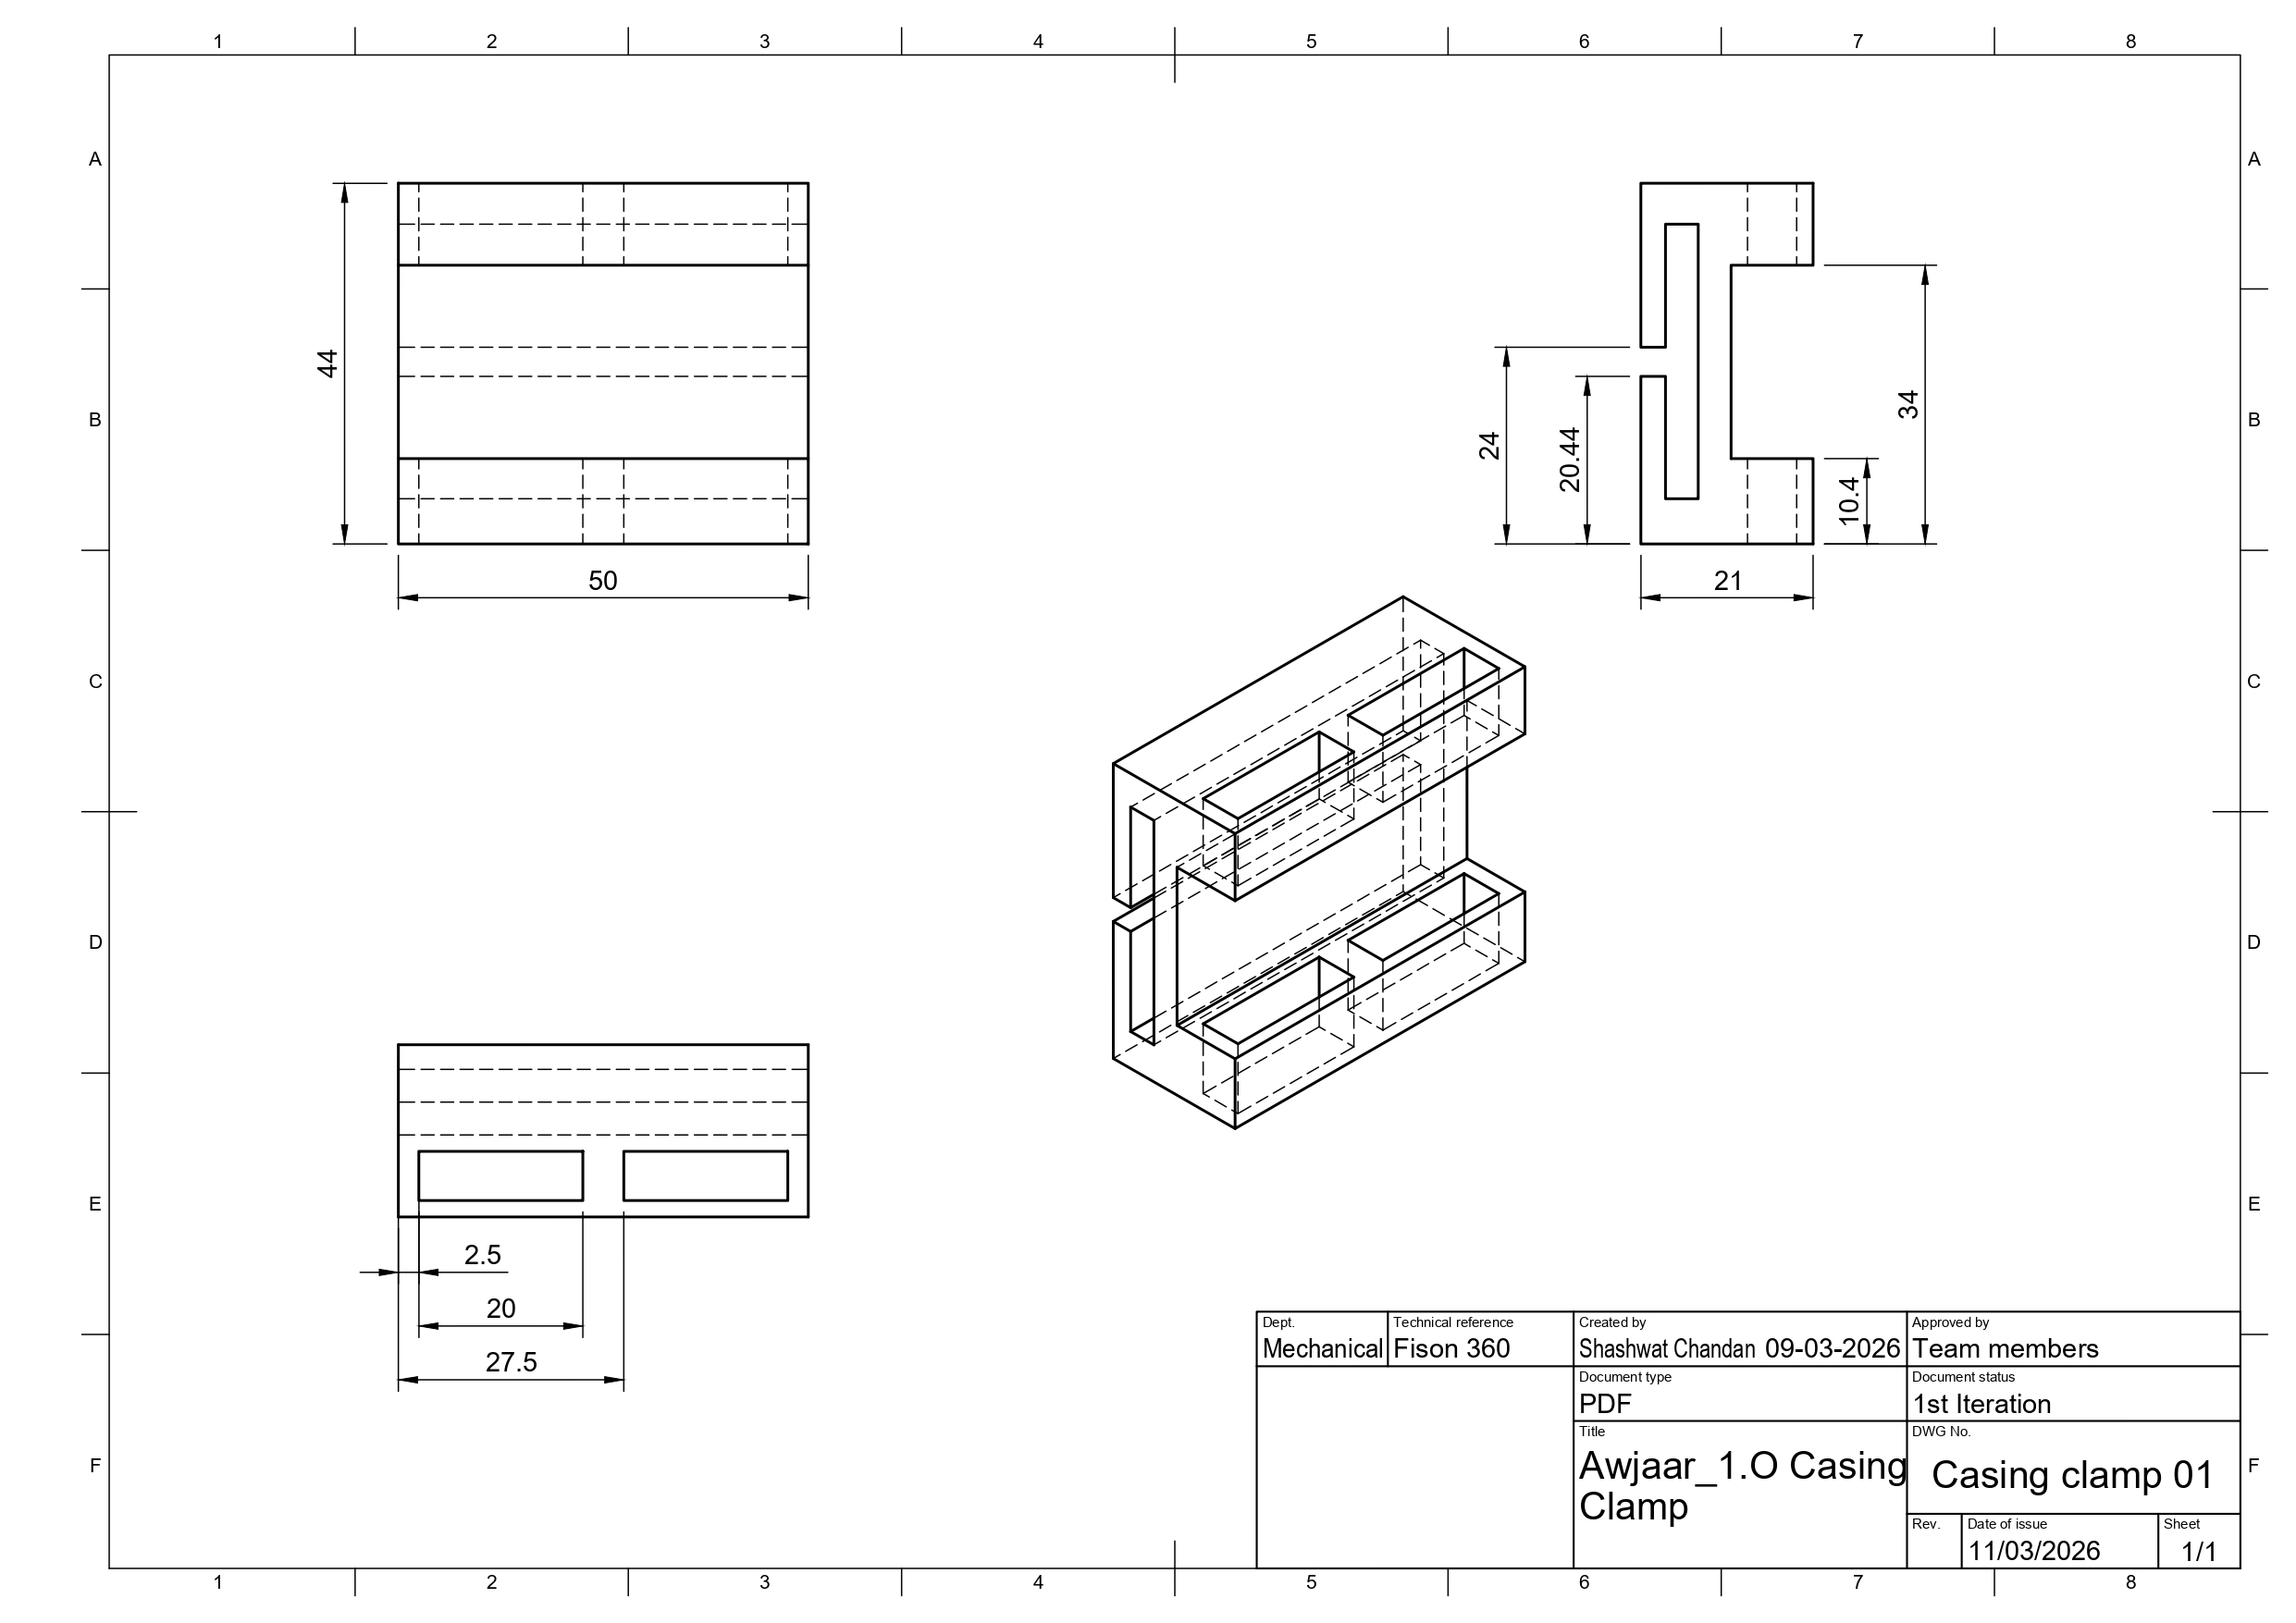
\includegraphics[width=\textwidth]{aujaar_2D_Clamp.jpg}
        \caption{AUJAR 2D clamp design}
    \end{subfigure}

    \vspace{0.5cm}

    \begin{subfigure}[b]{0.48\textwidth}
        \centering
        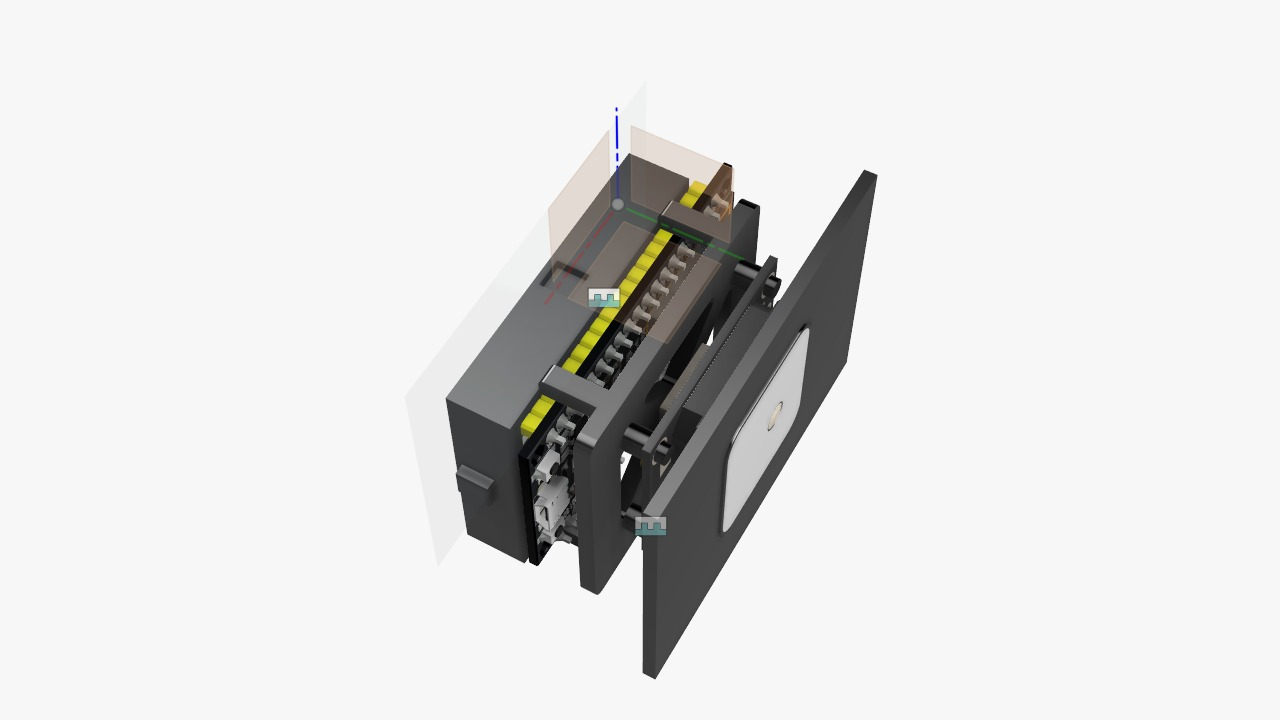
\includegraphics[width=\textwidth]{aujar_3d_model.jpeg}
        \caption{AUJAR 3D model}
    \end{subfigure}
    \hfill
    \begin{subfigure}[b]{0.48\textwidth}
        \centering
        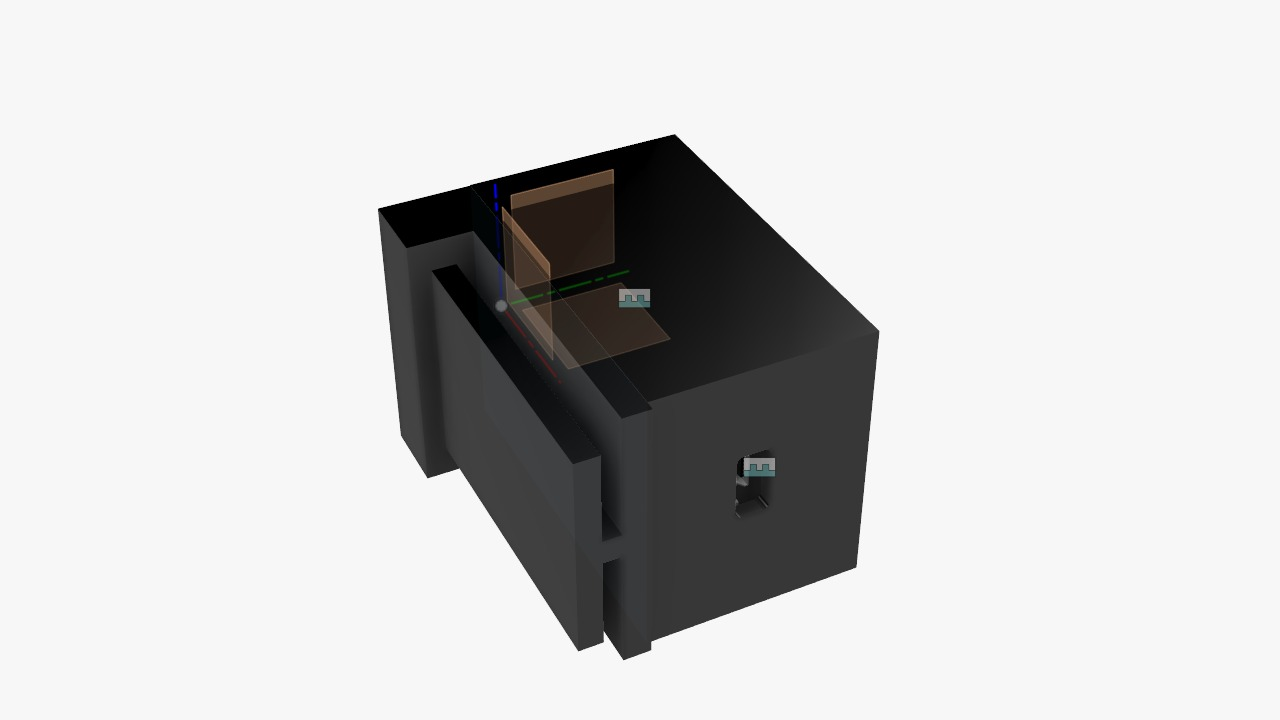
\includegraphics[width=\textwidth]{aujaar_mount_3d_model.jpeg}
        \caption{AUJAR mount 3D model}
    \end{subfigure}
    \caption{AUJAR hardware device --- 2D drawings and 3D models}
    \label{fig:aujar}
\end{figure}

\subsection{Solution Architecture}

The complete system is structured as a three-layer architecture with an optional hardware peripheral:

\begin{enumerate}[noitemsep]
    \item \textbf{Hardware Layer} --- AUJAR device acquires GPS coordinates and transmits via BLE.
    \item \textbf{Application Layer} --- Two React Native mobile apps (buyer and vendor), communicating with the server via REST API and Socket.io WebSockets.
    \item \textbf{Server Layer} --- A Node.js/Express bridge server backed by MongoDB for persistence and Socket.io for real-time event relay.
\end{enumerate}

The server uses JWT-based authentication for both REST and WebSocket channels. Vendor location data is persisted in MongoDB, and proximity filtering uses the Haversine formula to compute distances between GPS coordinates. The system maintains in-memory session maps and message queues so that requests and responses are not lost when either party is temporarily disconnected.

% ═══════════════════════════════════════════════════
% 5. BILL OF MATERIALS
% ═══════════════════════════════════════════════════
\section{Bill of Materials}

The Bill of Materials for the AUJAR hardware device is shown in Figure~\ref{fig:bom}. It includes the GPS module, BLE-capable microcontroller, battery, enclosure, and mounting hardware.

\begin{figure}[H]
    \centering
    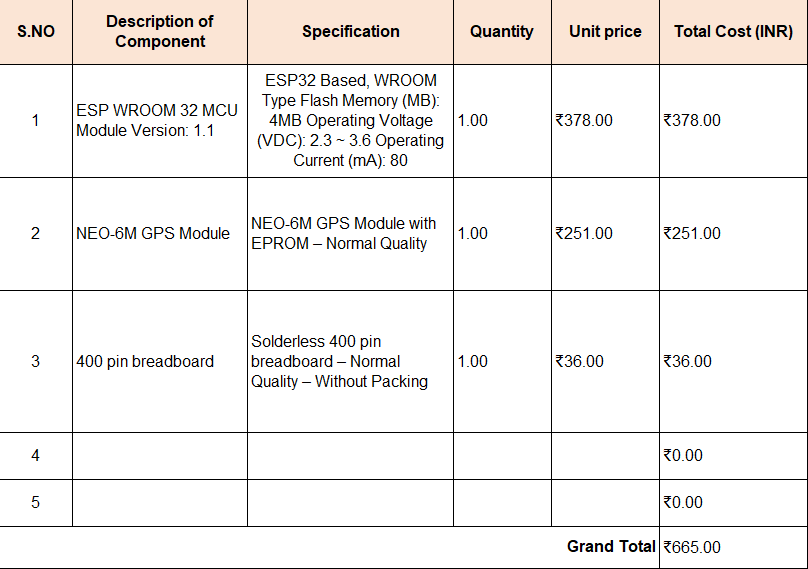
\includegraphics[width=0.95\textwidth]{BOM.png}
    \caption{Bill of Materials for the AUJAR device}
    \label{fig:bom}
\end{figure}

% ═══════════════════════════════════════════════════
% 6. PROTOTYPE
% ═══════════════════════════════════════════════════
\section{Prototype}

The working prototype consists of:

\begin{itemize}[noitemsep]
    \item A \textbf{Node.js bridge server} running Express for REST endpoints and Socket.io for real-time communication, connected to a MongoDB database.
    \item A \textbf{Vendor mobile application} (React Native / Expo) that allows vendors to register, manage inventory (add/edit/delete items), connect to GPS, broadcast their live location, and receive and respond to buyer requests.
    \item A \textbf{Buyer mobile application} (React Native / Expo) that allows buyers to register, view nearby broadcasting vendors on a dark-themed Leaflet map, search for vendors by product name or vendor ID, send item requests, and receive vendor responses with location pins.
\end{itemize}

\begin{figure}[H]
    \centering
    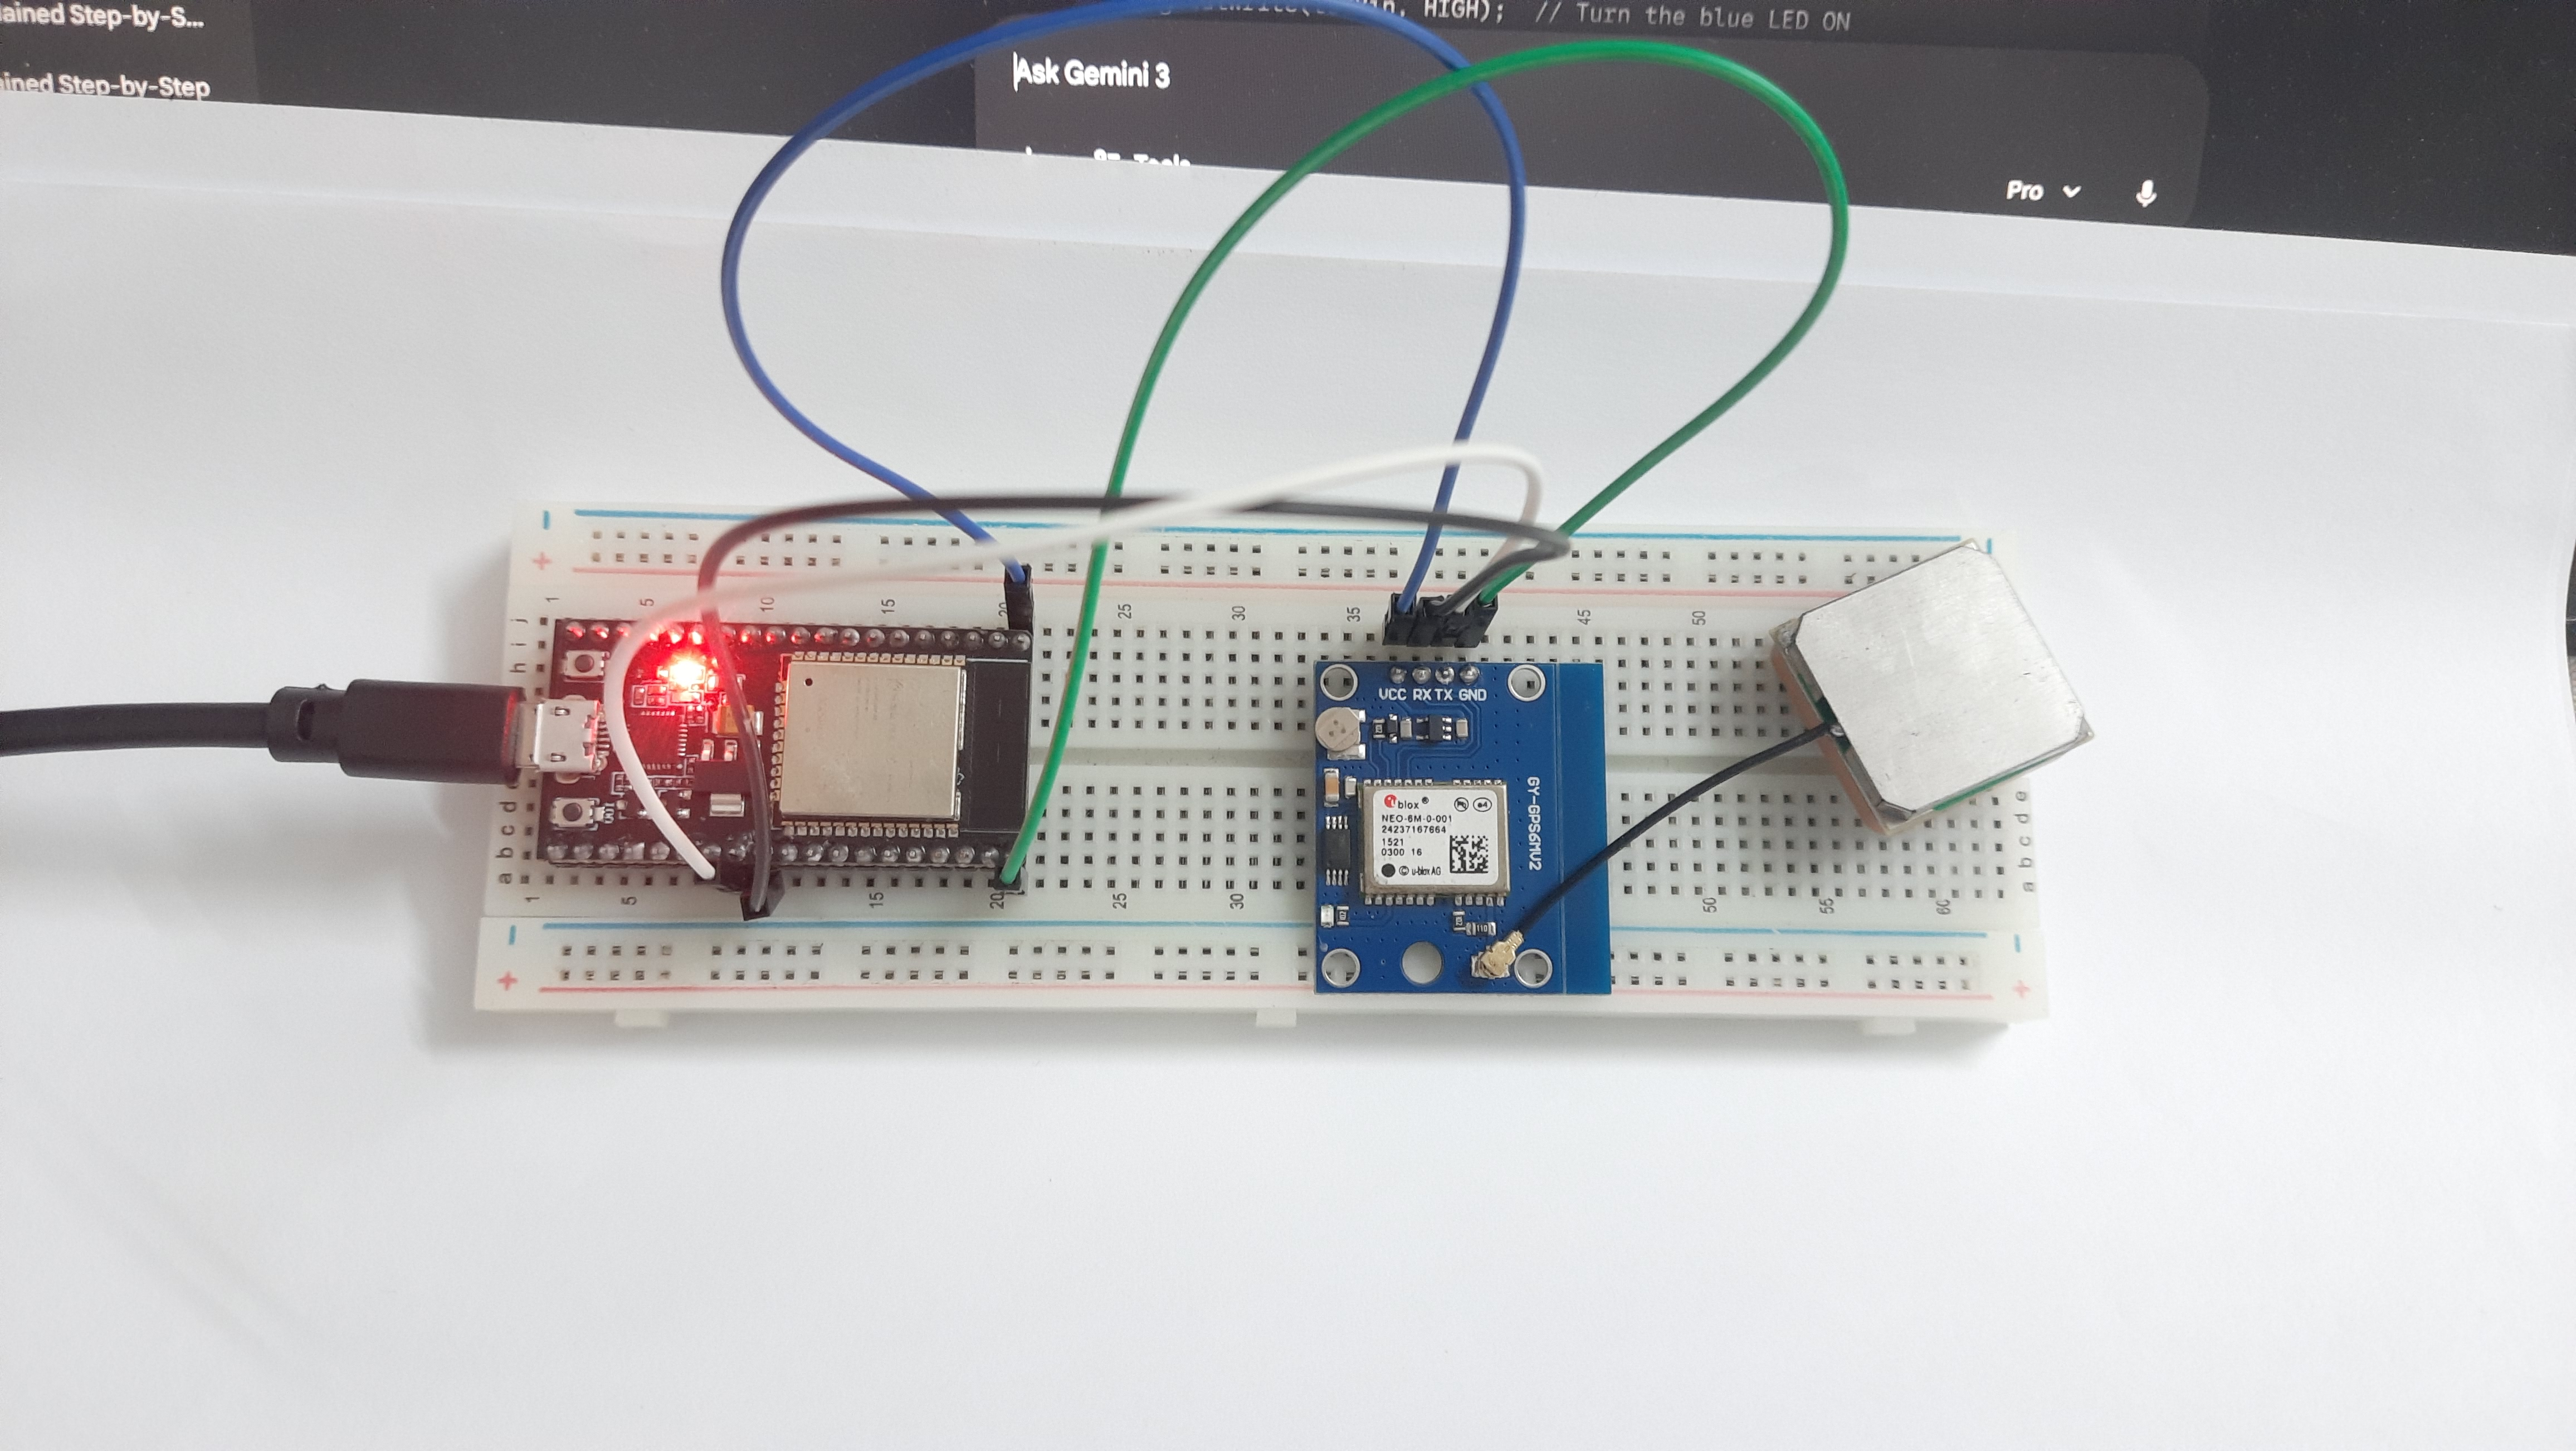
\includegraphics[width=0.6\textwidth]{prototype.jpeg}
    \caption{AUJAR hardware prototype}
    \label{fig:prototype}
\end{figure}

\subsection{Technology Stack}

\begin{table}[H]
    \centering
    \begin{tabularx}{\textwidth}{l l X}
        \toprule
        \textbf{Layer} & \textbf{Technology} & \textbf{Purpose} \\
        \midrule
        Server Runtime    & Node.js           & JavaScript runtime \\
        API Framework     & Express           & REST endpoint routing \\
        Real-time         & Socket.io         & WebSocket-based bidirectional communication \\
        Database          & MongoDB (Mongoose) & Persistent storage of vendors, clients, inventory \\
        Authentication    & JWT + bcrypt      & Token-based auth (7-day expiry), password hashing \\
        Mobile Framework  & React Native (Expo) & Cross-platform mobile apps (TypeScript) \\
        Maps              & Leaflet.js (WebView) & Dark-themed interactive maps with custom markers \\
        Location          & Expo Location     & Foreground GPS tracking on mobile \\
        \bottomrule
    \end{tabularx}
    \caption{Technology stack}
\end{table}

\subsection{Application Screenshots}

\begin{figure}[H]
    \centering
    \begin{subfigure}[b]{0.3\textwidth}
        \centering
        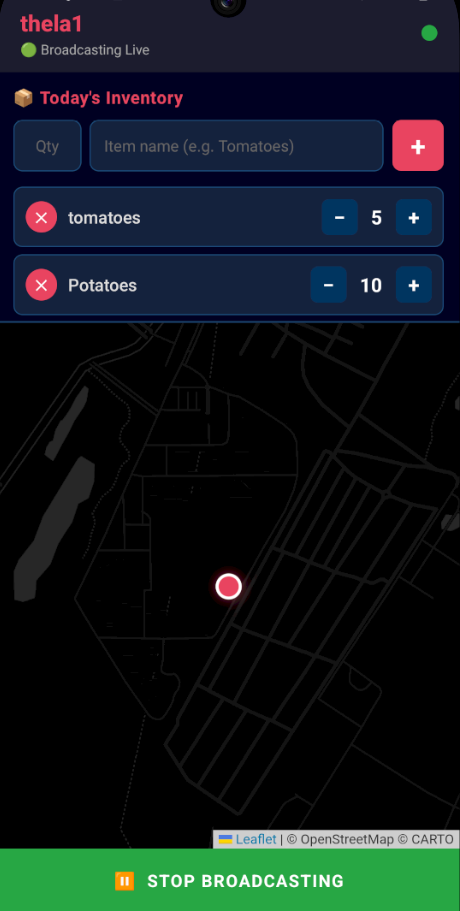
\includegraphics[width=\textwidth]{1_Vendor Home.png}
        \caption{Vendor home screen}
    \end{subfigure}
    \hfill
    \begin{subfigure}[b]{0.3\textwidth}
        \centering
        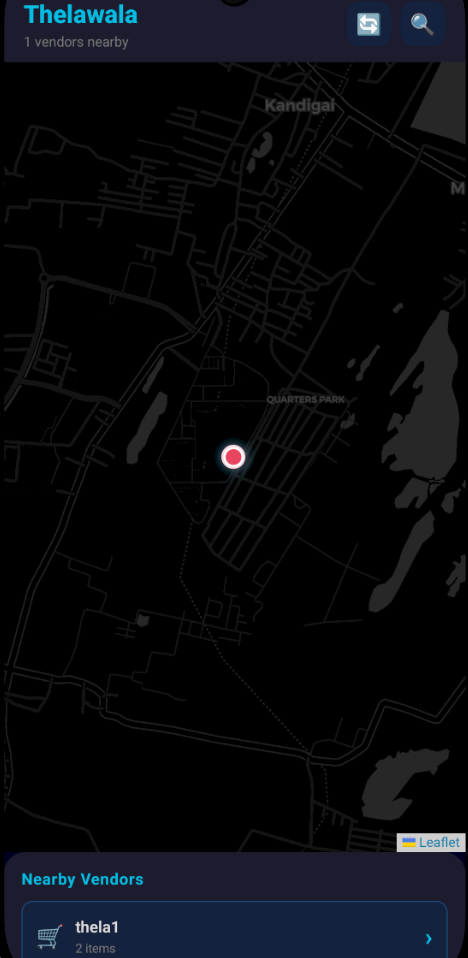
\includegraphics[width=\textwidth]{2_user vendor discovery.png}
        \caption{User discovers vendors}
    \end{subfigure}
    \hfill
    \begin{subfigure}[b]{0.3\textwidth}
        \centering
        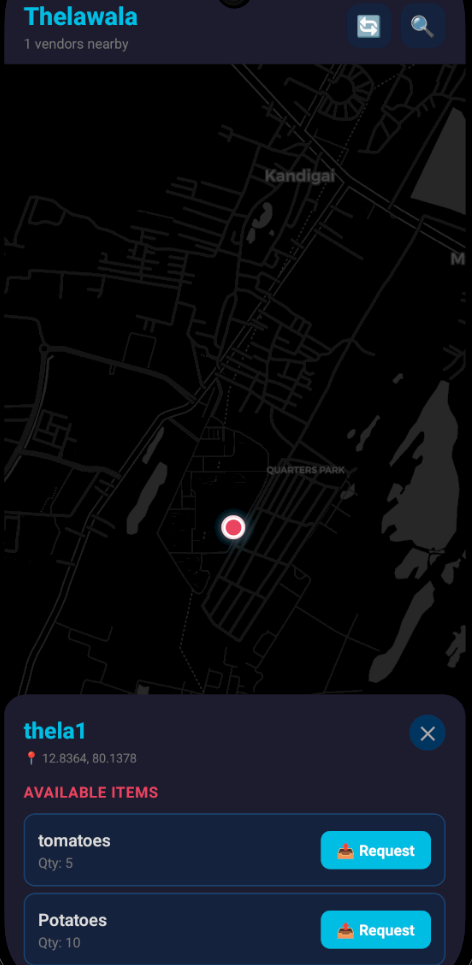
\includegraphics[width=\textwidth]{3_User stock Discovery.png}
        \caption{User views vendor stock}
    \end{subfigure}

    \vspace{0.5cm}

    \begin{subfigure}[b]{0.3\textwidth}
        \centering
        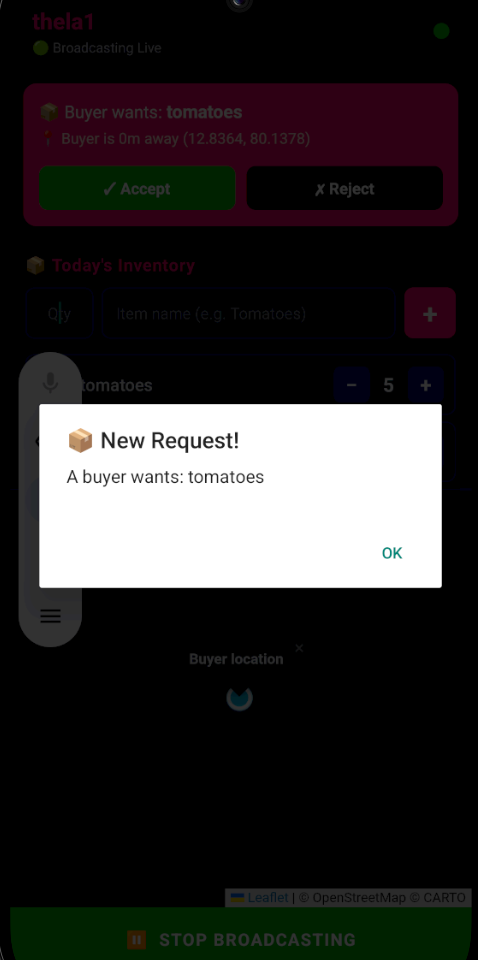
\includegraphics[width=\textwidth]{4_request recived by vendor.png}
        \caption{Vendor receives request}
    \end{subfigure}
    \hfill
    \begin{subfigure}[b]{0.3\textwidth}
        \centering
        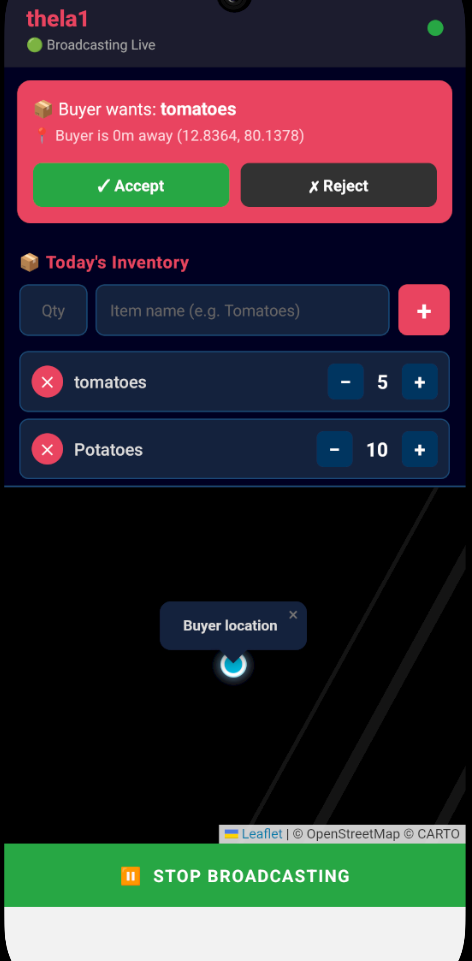
\includegraphics[width=\textwidth]{5_Vendor User Discovery.png}
        \caption{Vendor sees buyer location}
    \end{subfigure}
    \hfill
    \begin{subfigure}[b]{0.3\textwidth}
        \centering
        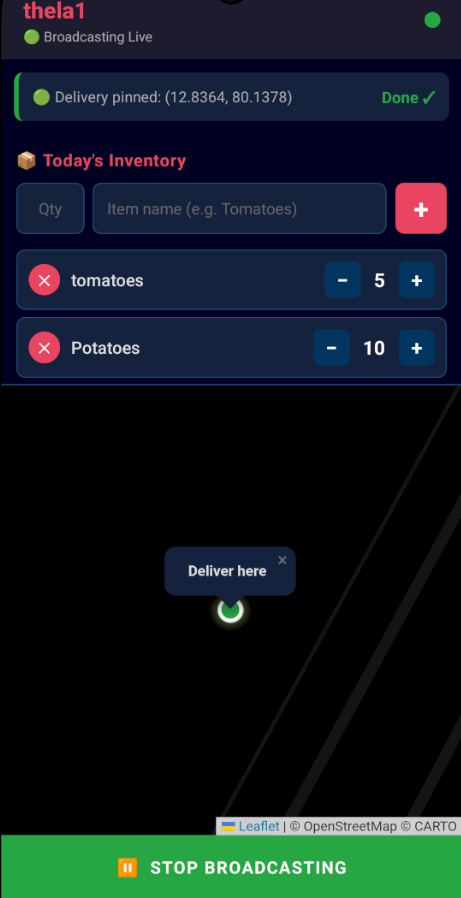
\includegraphics[width=\textwidth]{6_user delivery location.png}
        \caption{User sees vendor pin}
    \end{subfigure}
    \caption{Application screenshots showing the complete request--response flow}
    \label{fig:screenshots}
\end{figure}

\subsection{Key Implementation Details}

\textbf{Real-time Location Broadcast:} The vendor app acquires GPS coordinates every 5 seconds (1-metre distance threshold) and emits \texttt{vendor\_location\_update} events via Socket.io. The server persists the location and sets the vendor as ``broadcasting.''

\textbf{Nearby Vendor Discovery:} The buyer app polls the server every 15 seconds via a \texttt{get\_nearby\_vendors} socket event. The server queries all broadcasting vendors, filters them within a 5\,km radius using the Haversine formula, and returns the list.

\textbf{Item Request Routing:} When a buyer sends a request, the server looks up the vendor's active socket session. If the vendor is online, the request is delivered immediately; if not, it is queued in an in-memory pending-requests map and delivered upon reconnection.

\textbf{Grace Period Handling:} When a vendor's socket disconnects (e.g., app backgrounded), the server waits a configurable grace period before marking the vendor offline, preventing false ``0 vendors nearby'' results during brief disconnections.

% ═══════════════════════════════════════════════════
% 7. OUTCOME & INFERENCES
% ═══════════════════════════════════════════════════
\section{Outcome \& Inferences}

\subsection{Outcomes}

The prototype successfully demonstrates the core value proposition:

\begin{enumerate}[noitemsep]
    \item \textbf{Live vendor discovery} --- Buyers can see broadcasting vendors on a real-time map and discover them within a 5\,km radius.
    \item \textbf{Product-level search} --- Buyers can search by item name and receive a filtered list of vendors currently selling that product, or search directly by a vendor's Thela ID.
    \item \textbf{Purchase request flow} --- The complete request--accept/reject--location relay cycle works end-to-end. Accepted requests pin the vendor's location on the buyer's map.
    \item \textbf{Inventory management} --- Vendors can add, edit, and delete stock items with quantities; changes auto-sync to the server.
    \item \textbf{Offline resilience} --- Requests and responses are queued when either party is temporarily offline and delivered upon reconnection.
    \item \textbf{AUJAR abstraction} --- The vendor app's GPS layer is abstracted behind the \texttt{useAujarBluetooth} hook, providing a clean interface that can be swapped from phone GPS to actual BLE hardware with no changes to the rest of the application.
\end{enumerate}

\subsection{Inferences}

\begin{itemize}[noitemsep]
    \item The WebSocket-based architecture (Socket.io) provides low-latency real-time communication suitable for live GPS tracking and request routing.
    \item The Haversine-based proximity filter is effective for the current scale; spatial indexing (e.g., MongoDB geospatial queries) would be needed for larger deployments.
    \item The single-emulator testing scenario exposed the importance of grace-period handling and message queuing --- both were added to ensure reliable operation when apps are backgrounded.
    \item The concept of a dedicated hardware device (AUJAR) is validated at the architecture level: the software abstraction layer is in place and ready for hardware integration.
\end{itemize}

% ═══════════════════════════════════════════════════
% 8. FUTURE WORKS
% ═══════════════════════════════════════════════════
\section{Future Works \& Development}

\begin{enumerate}[leftmargin=*, noitemsep]
    \item \textbf{Automated Calling Service:} Integrate a telephony API (e.g., Twilio) to place automated voice calls to users when a subscribed vendor enters their proximity radius. This ensures notification delivery even on feature phones or when the app is closed.

    \item \textbf{Server Deployment:} Deploy the bridge server to a cloud platform (e.g., AWS, DigitalOcean) with a production-grade MongoDB Atlas cluster, HTTPS/TLS termination, and environment-based configuration. Migrate in-memory session and queue state to Redis for crash resilience and horizontal scalability.

    \item \textbf{AUJAR Device Configuration \& Packaging:} Complete the hardware prototype by integrating the GPS module and BLE-capable microcontroller onto a custom PCB, programming the firmware for continuous low-power GPS acquisition and BLE transmission, and packaging the electronics into the 3D-printed casing and clamp designs (Figure~\ref{fig:aujar}). The final device should mount securely onto a thela, operate for a full 8--12 hour work shift on a single charge, and require no user interaction beyond power-on.

    \item \textbf{Push Notifications:} Add Firebase Cloud Messaging for in-app alerts when the app is backgrounded.

    \item \textbf{Vendor Subscription / Follow:} Allow buyers to follow specific vendors and receive proximity-triggered notifications.

    \item \textbf{Community Relay Mode:} Enable a single phone to relay AUJAR GPS data from multiple nearby vendors simultaneously.

    \item \textbf{Order History \& Analytics:} Persist completed request records and provide vendors with insights on request acceptance rates, peak demand areas, and popular items.
\end{enumerate}

% ═══════════════════════════════════════════════════
% 9. REFERENCES
% ═══════════════════════════════════════════════════
\section{References}

\begin{enumerate}[noitemsep]
    \item Sneha, M., Praveen, K., Myna, K., \& Rithika, C. GPS Based Women Security System Using ESP32. \textit{International Journal of Innovative Research in Technology (IJIRT)}, 9(11), 221--224.
    \item Nauval, I., Widyanto, R.~A., Setiawan, A., Nuryanto, N., Prabowo, N.~A., \& Purnomo, T.~A. (2023). Implementation of GPS for tracking of street vendor. \textit{AIP Conference Proceedings}, 2702(1), 060006.
    \item Socket.io Documentation. \url{https://socket.io/docs/v4/}
    \item Express.js Documentation. \url{https://expressjs.com/}
    \item MongoDB Mongoose ODM. \url{https://mongoosejs.com/docs/}
    \item React Native (Expo) Documentation. \url{https://docs.expo.dev/}
    \item Leaflet.js --- Open-source interactive maps. \url{https://leafletjs.com/}
    \item JSON Web Tokens (JWT) Specification. RFC 7519. \url{https://datatracker.ietf.org/doc/html/rfc7519}
    \item Haversine Formula for GPS distance calculation. \url{https://en.wikipedia.org/wiki/Haversine_formula}
    \item React Native BLE PLX --- Bluetooth Low Energy library. \url{https://github.com/dotintent/react-native-ble-plx}
    \item Expo Location API. \url{https://docs.expo.dev/versions/latest/sdk/location/}
\end{enumerate}

\end{document}
